\documentclass[tikz]{standalone}
% https://rmwu.github.io/tutorial/latex/2019/08/27/intro/
\begin{document}

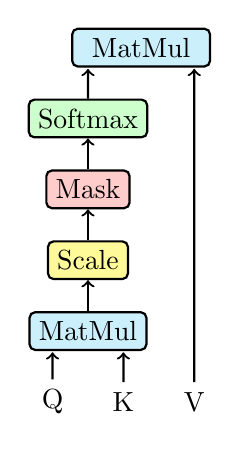
\begin{tikzpicture}[scale=0.9, every node/.append style={thick, rounded corners=2pt}]

\node (q) at (.5,0) {Q};
\node (k) at (1.5,0) {K};
\node (v) at (2.5,0) {V}; 

\node[draw, fill=cyan!20] (matmul1) at (1,1) {MatMul};
\node[draw, fill=yellow!40] (scale) at (1,2) {Scale};
\node[draw, fill=red!20] (mask) at (1,3) {Mask};
\node[draw, fill=green!20] (softmax) at (1,4) {Softmax};
\node[draw, fill=cyan!20, minimum width=1.75cm] (matmul2) at (1.75,5) {MatMul};

\path[->,thick]
    (matmul1) edge (scale)
    (scale) edge (mask)
    (mask) edge (softmax)
    (q) edge (0.5,0.7)
    (k) edge (1.5,0.7)
    (v) edge (2.5,4.7)
    (softmax) edge (1,4.7) 
    ;
\end{tikzpicture}

\end{document}
